\documentclass[a4paper,12pt]{extarticle}
\usepackage{geometry}
\usepackage[T1]{fontenc}
\usepackage[utf8]{inputenc}
\usepackage[english,russian]{babel}
\usepackage{amsmath}
\usepackage{amsthm}
\usepackage{amssymb}
\usepackage{fancyhdr}
\usepackage{setspace}
\usepackage{graphicx}
\usepackage{colortbl}
\usepackage{tikz}
\usepackage{pgf}
\usepackage{subcaption}
\usepackage{listings}
\usepackage{indentfirst}
\usepackage[
backend=biber,
style=numeric,
maxbibnames=99
]{biblatex}
\addbibresource{refs.bib}
\usepackage[colorlinks,citecolor=blue,linkcolor=blue,bookmarks=false,hypertexnames=true, urlcolor=blue]{hyperref} 
\usepackage{indentfirst}
\usepackage{mathtools}
\usepackage{booktabs}
\usepackage[flushleft]{threeparttable}
\usepackage{tablefootnote}

\usepackage{chngcntr} % нумерация графиков и таблиц по секциям
\counterwithin{table}{section}
\counterwithin{figure}{section}

\graphicspath{{graphics/}}%путь к рисункам

\makeatletter
% \renewcommand{\@biblabel}[1]{#1.} % Заменяем библиографию с квадратных скобок на точку:
\makeatother

\geometry{left=2.5cm}% левое поле
\geometry{right=1.0cm}% правое поле
\geometry{top=2.0cm}% верхнее поле
\geometry{bottom=2.0cm}% нижнее поле
\setlength{\parindent}{1.25cm}
\renewcommand{\baselinestretch}{1.5} % междустрочный интервал


\newcommand{\bibref}[3]{\hyperlink{#1}{#2 (#3)}} % biblabel, authors, year
\addto\captionsrussian{\def\refname{Список литературы (или источников)}} 

\renewcommand{\theenumi}{\arabic{enumi}}% Меняем везде перечисления на цифра.цифра
\renewcommand{\labelenumi}{\arabic{enumi}}% Меняем везде перечисления на цифра.цифра
\renewcommand{\theenumii}{.\arabic{enumii}}% Меняем везде перечисления на цифра.цифра
\renewcommand{\labelenumii}{\arabic{enumi}.\arabic{enumii}.}% Меняем везде перечисления на цифра.цифра
\renewcommand{\theenumiii}{.\arabic{enumiii}}% Меняем везде перечисления на цифра.цифра
\renewcommand{\labelenumiii}{\arabic{enumi}.\arabic{enumii}.\arabic{enumiii}.}% Меняем везде перечисления на цифра.цифра

\begin{document}
\begin{titlepage}
\newpage

{\setstretch{1.0}
\begin{center}
ПРАВИТЕЛЬСТВО РОССИЙСКОЙ ФЕДЕРАЦИИ\\
ФГАОУ ВО НАЦИОНАЛЬНЫЙ ИССЛЕДОВАТЕЛЬСКИЙ УНИВЕРСИТЕТ\\
«ВЫСШАЯ ШКОЛА ЭКОНОМИКИ»
\\
\bigskip
Факультет компьютерных наук\\
Образовательная программа «Прикладная математика и информатика»
\end{center}
}

\vspace{2em}
УДК 004.8 % УДК нужно указывать только для исследовательсвого проекта - удалите эту строку для программного проекта
\vspace{5em}

\begin{center}
%Выберите какой у вас проект
{\bf Отчет об исследовательском проекте на тему:}\\
%{\bf Отчет о программном проекте на тему:}\\
{\bf Кластеризация аудио}\\
(промежуточный, этап 1)
\end{center}

\vspace{2em}

{\bf Выполнил студент: \vspace{2mm}}

{\setstretch{1.1}
\begin{tabular}{l@{\hskip 1.5cm}l}
группы \#БПМИ213 & Бонич Дмитрий Сергеевич 
\end{tabular}}

\vspace{1em}
{\bf Принял руководитель проекта: \vspace{2mm}}

{\setstretch{1.1}
\begin{tabular}{l}
Сендерович Александра Леонидовна\\
Научный сотрудник\\
Факультет компьютерных наук НИУ ВШЭ 
\end{tabular}}

\vspace{\fill}

\begin{center}
Москва 2024
\end{center}

\end{titlepage}
% это титульный лист - выберите подходящий вам из имеющихся в проекте вариантов
\newpage
\setcounter{page}{2}

{
	\hypersetup{linkcolor=black}
	\tableofcontents
}

\newpage

\newpage
\section*{Аннотация}   % this is how to use russian
    Существующие методы глубинного обучения для кластеризации 
    изображений работают довольно хорошо. Однако вопрос качественной
    кластеризации аудио остается открытым. В этой работе мы планируем
    адаптировать лучшие методы кластеризации изображений для 
    задачи кластеризации аудио.

\addcontentsline{toc}{section}{Аннотация}

\section*{Ключевые слова}
Глубинное обучение, обучение без учителя, кластеризация
\pagebreak

\section{Введение}

\subsection{Постановка задачи}

В задаче классификации мы имеем обучающую выборку, где для каждого объекта
известен его класс и от нас требуется моделировать распределение
классов на пространстве объектов. Задача кластеризации более сложная
-- необходимо разбить объекты на осмысленные группы не зная ни 
самих групп, ни их распределения.

\subsection{Метрики качества}

Чтобы замерить качество кластеризации как правило метод
решает задачу на размеченном для кластеризации датасете, 
разумеется не используя метки классов. Полученные после 
кластеризации номера кластеров будем называть \textit{псевдометками}.
Псевдометки сравниваются с настоящими метками
и качество определяется как некоторый вид корреляции между ними.

Одной из самых популярных метрик качества является NMI(Normalized Mutual Information).
Пусть у нас есть пара случайных величин $X$ и $Y$, тогда:

\[
	\text{NMI}(X,Y) = \frac{\text{KL}(p_{(X, Y)}| p_X \otimes p_Y)}{\sqrt{H(X)H(Y)}}
\]
При подсчете NMI мы считаем распределения меток и псевдометок 
за $X$ и $Y$ и вычисляем \textit{оценку максимального правдоподобия}\footnote{далее ОМП}. NMI 
принимает значения от 0 до 1.

Еще одной используемой метрикой является ARI(Adjusted Rand Index).
Это скорректированная версия метрики RI\footnote{\url{https://en.wikipedia.org/wiki/Rand_index}} (Rand Index).
Определяется ARI следующим образом:

\[
	\text{ARI}(X, Y) = \frac{\text{RI}(X, Y) - \text{E}[\text{RI}(X, Y)]}{1 - \text{E}[\text{RI}(X, Y)]}
\]

ARI принимает значения от 0 до 1.

Также в качестве метрики качества можно использовать долю 
правильных ответов как и в задаче классификации. Однако предварительно 
необходимо решить \textit{задачу о назначениях}\footnote{\url{https://en.wikipedia.org/wiki/Assignment_problem}}.
между псевдометками и метками.
Мы переименуем псевдометки так, чтобы достичь максимального качества.
Затем на переименованных псевдометках мы посчитаем долю правильных ответов, которую 
и используем в качестве метрики качества.

\subsection{Классические методы решения}

С точки зрения классических методов кластеризуемые
объекты это точки в многомерном пространстве. Такие
методы обычно имеют итерационную природу и решают 
задачу выделения кластеров точек находя их скопления, 
области с повышенной плотностью, некоторые структуры.
Приведем пример такого метода.

\subsubsection{K-means}

Одним из самых простых и известных методов является
K-means. Он работает на базе EM-алгоритма\footnote{\url{https://en.wikipedia.org/wiki/Expectation\%E2\%80\%93maximization_algorithm}}.
K-means итерационно пытается найти два неизвестных набора переменных ---
номера кластеров для объектов и центры этих кластеров. 
Количество кластеров фиксировано и задается до начала 
работы алгоритма в качестве гиперпараметра $k$.

В начале своей работы классический K-means инициализирует все 
центры кластеров случайно. Затем чередуются E и M шаги до 
сходимости. На E-шаге мы назначаем каждому объекту номер
кластера к центру которого объект ближе всего в качестве псевдометки.
На M-шаге мы вычисляем ОМП для каждого центра кластера, то есть 
берем в качестве центра кластера усредненную точку из всех объектов 
с псевдометкой этого кластера.

\section{Обзор литературы}

При кластеризации сложных объектов таких как изображения или 
аудио недостаточно вытянуть данные объекта в вектор и применить
классический алгоритм кластеризации для полученных точек. 
Чтобы алгоритмы кластеризации хорошо работали входное 
пространство точек должно обладать некоторыми свойствами.
В идеале близкие в этом пространстве точки должны принадлежать 
к одной группе.

Таким образом задачу кластеризации сложных объектов можно 
разделить на две части -- получение представлений объектов 
образующих пригодное для кластеризации пространство точек и 
сама кластеризация этих представлений. Метод переводящий объекты
в признаки будем называть \textit{энкодером}.

\subsection{DeepCluster}

Одним из первых методов использующих глубинное обучения для 
кластеризации изображений был
DeepCluster \cite{Caron_2018_ECCV}. DeepCluster использует 
сверточную нейросеть $f_\theta$ в качестве энкодера.
К полученным признакам применяется K-means и мы получаем
псевдометку $y_n$ для каждого изображения $x_n$. Затем к 
сверточной сети прикрепляется
классификационная голова $g_W$. $g_W$ предсказывает 
вероятности кластеров для объекта по его признакам 
полученным из $f_\theta$. Псевдометки используются как настоящие для подсчета логистической 
функции потерь. Таким образом мы решаем следующую задачу 
оптимизации:

\[
	\min_{\theta, W} \frac{1}{N}\sum_{n=1}^N 
	l(g_W(f_\theta(x_n)), y_n)
\]

Здесь $N$ -- это размер батча, $l$ логистическая 
мультиномиальная функция потерь

По усредненному значению функции потерь для батча делается проход назад и веса 
$\theta$ и $W$ обновляются стохастическим градиентным спуском. Затем 
шаги кластеризации и оптимизации параметров сети повторяются 
заданное количество эпох.

Однако в такой постановке метод выраждается в тривиальные 
решения. Их существует 2 типа - пустые кластеры и 
тривиальная параметризация

Чтобы не допустить возникновения пустых кластеров 
сделаем следующую модификацию K-means. Пусть 
на некоторой итерации у нас появился пустой 
класс A. Тогда возьмем случайный непустой класс 
B. Добавим к центру B шум получив новый центр 
для кластера A. Переназначим классы точек из B 
так чтобы каждая точка имела класс ближайшего 
центра кластера. 

Тривиальная параметризация возникает когда 
распределение классов становится сильно неравномерным. 
Тогда классификационной голове становится выгодно выдавать 
только несколько наиболее часто встречающихся классов игнорируя остальные. 
Чтобы этого избежать необходимо сэмплировать объекты для батча 
из равномерного распределения по псевдометкам с предыдущего шага.

\subsection{SPICE}

SPICE предложенный в \cite{niu2021spice} является более 
продвинутым методом нежели DeepCluster и имеет лучшее качество.
Целью SPICE является обучение энкодера и кластеризационной головы. 
В качестве энкодера используется сверточная нейросеть.
Кластеризационная голова это двухслойный MLP(Multilayer perceptron). 
Она принимает на вход признаки из энкодера и выдает вероятности 
кластеров.

Метод состоит из 3-ех этапов. На первом этапе обучается энкодер.
На втором этапе энкодер фиксируется и обучается только кластеризационная
голова. На третьем этапе энкодер и кластеризационная голова обучаются 
вместе. 

\begin{figure}[ht]
	\centering
	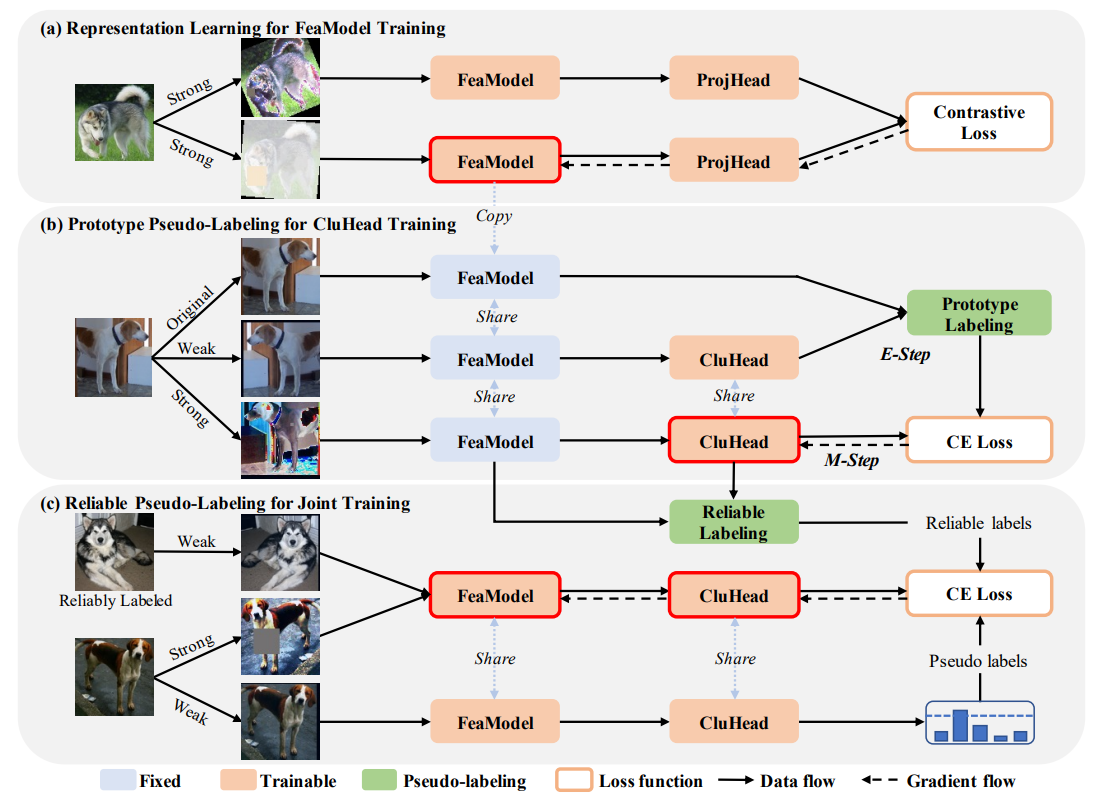
\includegraphics[width=0.8\textwidth]{spice.png}
	\caption{Этапы обучения метода SPICE. 
	FeaModel - энкодер, ProjHead - проекционная голова, CluHead - кластеризационная голова. a) Обучение энкодера. b) Обучение кластеризационной головы.
	с) Совместное обучение энкодера и кластеризационной головы. }
	\label{fig:spice}
\end{figure}

Схематический принцип работы каждого этапа можно видеть 
на Рисунке~\ref{fig:spice}. Перейдем к разбору каждого этапа
по отдельности.

\subsubsection{Обучение энкодера}

Помимо энкодера будем учить проекционною голову, которая 
представляет из себя двухслойный MLP. Как показано на 
Рисунке~\ref{fig:spice}(a) мы копируем энкодер и 
кластризационную голову, чтобы получить две ветки 
для обучения. 

На вход веткам подаются разные аугментации одного и того же 
изображения. Аугментированное изображение проходит через энкодер соответствующей
ветки и полученные признаки подаются на вход проекционной голове
из той же ветки. В итоге из верхней и нижней веток мы 
получаем вектора $z^{+}$ и $z$ соответственно. После 
этого мы считаем следующую функцию потерь:

\[
	\mathcal{L}_{fea} = -\ln\left(
		\frac{\exp(z^T z^{+}/\tau)}
		{\sum_{i=1}^{N_q}\exp(z^T z_i^{-}/\tau) + 
		\exp(z^T z^{+}/\tau)}
	\right)
\]

Здесь за $z_i^{-}$ обозначены результаты верхней ветки для 
любых изображений отличных от текущего. Мы поддерживаем 
очередь из последних $N_q$ таких негативных примеров. $\tau>0$ --
гиперпараметр температуры.

С помощью посчитанной функции потерь $\mathcal{L}_{fea}$ 
мы делаем проход назад по нижней ветке и делаем шаг 
градиентного спуска. Верхняя ветка 
обновляется как экспоненциально движущееся среднее\footnote{\url{https://en.wikipedia.org/wiki/Moving\_average\#Exponential\_moving\_average}} 
нижней.

\textbf{Замечание.} На самом деле вместо описанного 
алгоритма можно использовать любой метод обучения представлений
для изображений без учителя.

\subsubsection{Обучение кластеризационной головы}

Энкодер на этом этапе фиксирован и не обучается. 
На данном этапе у нас есть два набора неизвестных переменных:
оптимальные параметры кластеризационной головы и правильные назначения 
классов объектам. Поэтому для их нахождения мы можем воспользоваться ЕМ-алгоритмом.
На Е-шаге мы будем считать параметры кластеризационной головы известными 
и будем искать назначения кластеров объектам. На М-шаге мы будем 
считать известными назначения кластеров и будем оптимизировать параметры 
кластеризационной головы. Рассмотрим подробно эти 2 шага.

На Е-шаге мы сначала вычисляем признаки $f_i$ из 
верхней ветки Рисунок~\ref{fig:spice}(b). С помощью 
средней ветки мы получаем вероятности каждого кластера для 
каждого объекта из батча. Для каждого кластера мы выбираем 
топ $\frac{M}{K}$ объектов с максимальными 
вероятностями полученными из второй ветки и берем их признаки
$f_i$ как показано в \ref{eq:prototype_cluster_features}.
\begin{align}\label{eq:prototype_cluster_features}
	\mathfrak{F}_k=\left\{f_i\Big\vert i\in\text{argtopk}\left(P_{:,k}, \frac{M}{K}\right), 
	\forall i=1, \ldots, M \right\}
\end{align}

Здесь $M$ это 
размер батча, а $K$ количество кластеров задаваемое как 
гиперпараметр до начала работы алгоритма. $P$ это матрица
вероятностей где по строкам разложены вероятности кластеров 
для каждого объекта из батча.

Далее для 
каждого класса $k$ мы вычисляем его центр $\gamma_k$, 
как среднее по точкам из $\mathfrak{F}_k$. Затем 
мы вычисляем косинусную похожесть между признаками $f_i$ 
и центрами кластеров $\gamma_k$. За $\mathfrak{X}^k$ обозначим 
$\frac{M}{K}$ ближайших в данной метрике объектов к 
центру кластера $\gamma_k$. Скажем что все объекты 
в $\mathfrak{X}^k$ имеют одну и туже псевдометку, а именно 
$y_i^s=k\quad \forall x_i\in\mathfrak{X}^k$. Результатом 
E-шага будет следующее множество пар объект-псевдометка:
\[
	\mathfrak{X}^s=\{(x_i, y_i^s)\mid \forall x_i 
	\in \mathfrak{X}^k, k=1,\ldots, K \}
\]

Будем называть псевдометки из $\mathfrak{X}^s$ протопсевдометками.

Перейдем к M-шагу. Используя протопсевдометки с Е-шага и вероятности 
классов полученные из нижней ветки мы можем посчитать следующую функцию 
потерь:
\[
	\mathcal{L}_{clu}=\frac{1}{M}\sum_{i=1}^M L_{ce}(y_i^s, p_i')
\]

Здесь $L_{ce}$ это логистическая функция потерь, $p_i'=\text{softmax}(p_i)$. 
$p_i$ это вероятности полученные из нижней ветки. Стоит заметить, что в итоге к 
логитам из нижней ветки два раза применяется операция softmax. Авторы 
обосновывают такое решение тем, что двойной softmax замедляет процесс обучения. 
Таким образом такая функция потерь меньше доверяет протопсевдометкам, 
что особенно полезно в начале обучения. 

Функция потерь $\mathcal{L}_{clu}$ используется для прохода назад 
через кластеризационную голову. Затем делается шаг градиентного спуска.

Можно заметить что 2-ой этап довольно легковесный т. к. нам необходимо 
обучать только кластеризационную голову с малым количеством параметров. 
Поэтому авторы предлагают параллельно учить сразу несколько голов и выбирать
лучшую по функции потерь $\mathcal{L}_{clu}$ для уменьшения дисперсии решения.

Стоит также обратить внимание, что распределения аугментаций 
для разных веток отличаются. Как видно на рисунке \ref{fig:spice}(b) 
верхней ветке на вход подается оригинал изображения, средней ветке
слабо аугментированое изображение, а нижней сильно аугментированное.

\subsubsection{Совместное обучение энкодера и кластеризационной головы}

На данном этапе мы хотим дообучить энкодер и кластеризационную голову.
С Е-шага прошлого этапа мы можем получить набор $\{x_i, f_i, y_i^s\}_{i=1}^N$, 
где $N$ это размер выборки. Для каждого объекта $x_i$ 
выберем $N_s$ ближайших соседей по косинусной похожести, 
обозначим метки объектов каждого такого множества за 
$\mathfrak{L}_i$. Введем величину $r_i$:
\[
	r_i=\frac{1}{N_s}\sum_{y\in \mathfrak{L}_i}I(y=y_i^s)
\]

Введем гиперпараметр порога $\lambda$. Если 
$r_i>\lambda$, то будем считать такой объект надежно 
размеченным, иначе нет. Таким образом подмножество 
надежно размеченных объектов $\mathfrak{X}^r$ определяется 
следующим образом:
\[
	\mathfrak{X}^r=\{(x_i, y_i^s)\mid r_i>\lambda, 
	\forall i = 1, \ldots, N\}
\]

Во время обучения полученные надежные псевдометки
фиксируются.

Затем каждую эпоху мы вычисляем консистентные псевдометки:
\[
	y_j^u=\begin{cases}
		\text{argmax}(p_j) & \text{если } max(p_j)\geq \eta, \\
		-1 & \text{иначе}	
	\end{cases}
\]

Здесь $p_j$ вероятности кластеров для объекта $j$ получены
после прогонки слабой аугментации объекта через энкодер 
и кластеризационную голову Рисунок~\ref{fig:spice}(c).
$\eta$ гиперпараметр порог. Теперь мы можем посчитать 
следующий функционал ошибки:

\[
	\mathcal{L}_{joint} = \frac{1}{L} \sum_{i=1}^L 
	\mathcal{L}_{ce}(y_i^s, \mathcal{C}(\mathcal{F}(\alpha(x_i))))
	+\frac{1}{U}\sum_{i=1}^U \mathbb{I}(y_j^u\geq 0) 
	\mathcal{L}_{ce} (y_j^u, \mathcal{C}(\mathcal{F}(\beta(x_j))))
\]

Тут первое слагаемое отвечает за надежно размеченные сэмплы 
и их количество равняется $L$. Второе слагаемое отвечает 
за сэмплы с консистентыми псевдометками и их количество 
равняется $U$. $\mathcal{F}$ и $\mathcal{C}$ это 
энкодер и кластеризационная голова соответственно. 
$\alpha$ и $\beta$ это слабая и сильная аугментации соответственно.

С помощью $\mathcal{L}_{joint}$ делается проход назад и шаг градиентного 
спуска по параметрам энкодера и кластеризционной головы.

\textbf{Замечание.} После получения надежных псевдометок 
можно применить любой метод частичного обучения\footnote{\url{https://en.wikipedia.org/wiki/Weak\_supervision\#Semi-supervised\_learning}}.

\subsection{Случай аудио}

Рассмотренные раннее методы занимаются кластеризацией 
изображений. Однако их можно адаптировать для кластеризации 
аудио. Для этого каждую аудиозапись можно перевести в 
изображение отражающее его структуру -- спектрограмму\footnote{\url{https://en.wikipedia.org/wiki/Spectrogram}}.
Так например DeepCluster был адаптирован для аудио как 
DECAR \cite{Ghosh2022DECARDC}.

\section{План дальнейшей работы}

В дальнейшем планируется выбрать размеченный аудио 
датасет и построить бейзлайн для кластеризации. Он будет 
устроен следующим образом. Некоторому энкодеру на вход 
будет подаваться спектрограмма. Полученные признаки будут 
уменьшены некоторым методом уменьшения размерности, например
PCA\footnote{\url{https://en.wikipedia.org/wiki/Principal\_component\_analysis}}. Затем малоразмерные признаки будут 
кластеризованны некоторым классическим методом, например 
K-means. Планируется добавить в бейзлайн несколько различных
комбинаций (энкодер, метод уменьшения размерности, метод 
кластеризации). В качестве основных метрик качества планируется
использовать NMI и долю правильных ответов. После этого 
планируется адаптировать метод SPICE для аудио и возможно 
другие новые методы кластеризации изображений и сравнить их 
с бейзлайном. 
	
\newpage 
\printbibliography[heading=bibintoc] 
	
\end{document}
